\documentclass{standalone}
\standaloneconfig{border=2mm 2mm 2mm 2mm}
\usepackage{tikz}
\usetikzlibrary{calc} 
\begin{document}

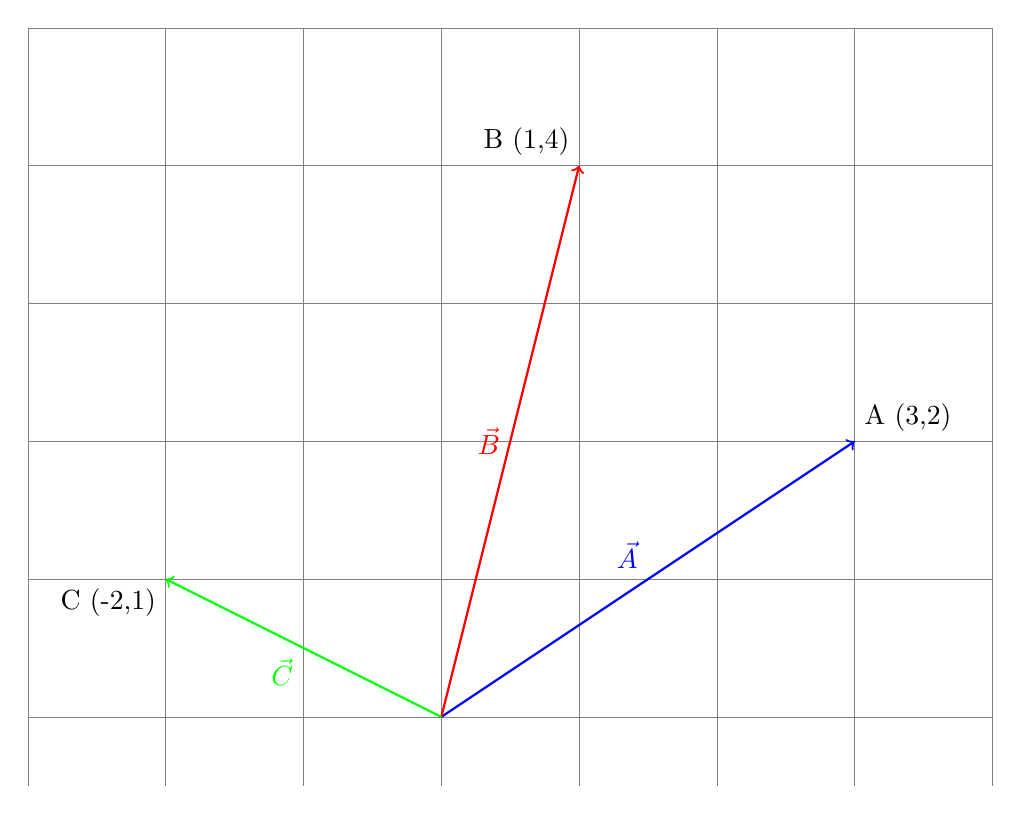
\begin{tikzpicture}[scale=1.75]
    \draw [help lines] (-3,-0.5) grid (4,5);
    % Three vectors, A, B, and C, and their resultant, R.
    % Define the origin
    \coordinate (O) at (0,0);
    
    % Define vectors A, B, and C by their terminal points
    \coordinate (A) at (3,2);    % Vector A from (0,0) to (3,2)
    \coordinate (B) at (1,4);    % Vector B from (0,0) to (1,4)
    \coordinate (C) at (-2,1);   % Vector C from (0,0) to (-2,1)
    
    % Draw vectors A, B, C from the origin
    \draw[->, thick, blue] (O) -- (A) node[midway, above left] {$\vec{A}$};
    \draw[->, thick, red] (O) -- (B) node[midway, left] {$\vec{B}$};
    \draw[->, thick, green] (O) -- (C) node[midway, below left] {$\vec{C}$};
    
    % Add labels for the points
    \node at (A) [above right] {A (3,2)};
    \node at (B) [above left] {B (1,4)};
    \node at (C) [below left] {C (-2,1)};

\end{tikzpicture}

\end{document}
